\section{Methodology}

We propose \textit{SegviGen}, a unified multi-task framework for 3D part segmentation that supports three practical settings: interactive part-segmentation, full segmentation, and full segmentation with 2D guidance.
%
To leverage the prior knowledge encoded in a pretrained 3D generative model, we cast 3D segmentation as a colorization problem.
%
Specifically, we encode the input 3D asset into a compact latent that conditions generation, and optionally augment it with user interactions or a 2D segmentation map.
%
Conditioned on these inputs, the model reconstructs the 3D asset while predicting colors for active voxels in the structured 3D representation, where each color corresponds to an individual part, yielding the final segmentation.
%
Below, we begin by describing the underlying 3D generative model (Sec.~\ref{sec:3d_generative_model}), followed by our task reformulation (Sec.~\ref{sec:task_define}), and then detail the overall pipeline (Sec.~\ref{sec:pipeline}).


\subsection{Preliminary: Structured 3D Generative Model}
\label{sec:3d_generative_model}

Recent work~\cite{trellis2} organizes each textured 3D asset into a sparse set of active voxels on a regular grid, where every active voxel stores geometry and texture features aligned in 3D.
%.
This formulation leverages a flexible dual-grid construction to robustly handle arbitrary topology while encoding physically-based material attributes jointly with geometry for faithful appearance modeling.
%
Given the sparse omni-voxel representation, a Sparse Compression VAE (SC-VAE) maps each voxelized asset feature tensor $\mathbf{x}$ to a compact structured latent $\mathbf{z}_1=E_{\phi}(\mathbf{x})$ and reconstructs it via $\hat{\mathbf{x}}=D_{\theta}(\mathbf{z}_1)$, yielding an expressive yet highly compressed 3D latent space.
%
On top of these latents, a conditional flow-matching generator learns a time-dependent vector field $\mathbf{v}_{\psi}(\mathbf{z}_t,t,\mathbf{c})$ under conditioning $\mathbf{c}$ by matching the constant velocity along linear interpolants:
\begin{equation}
\mathbf{z}_0\sim\mathcal{N}(\mathbf{0},\mathbf{I}),\quad t\sim\mathcal{U}(0,1),\quad \mathbf{z}_t=(1-t)\mathbf{z}_0+t\mathbf{z}_1,
\end{equation}
\begin{equation}
\mathcal{L}_{\mathrm{cfm}}
=\mathbb{E}\Big[\big\|\mathbf{v}_{\psi}(\mathbf{z}_t,t,\mathbf{c})-(\mathbf{z}_1-\mathbf{z}_0)\big\|_2^2\Big].
\end{equation}
%
This latent generative pipeline enables efficient synthesis of geometry- and texture-consistent 3D assets, 
and the resulting structured latents capture rich joint statistics of shape and appearance, providing a strong transferable prior for fine-grained 3D part segmentation.


\subsection{Task Reformulation and I/O Representation}
\label{sec:task_define}

We reformulate 3D part segmentation as a color prediction problem in a structured 3D representation.
%
This choice matches our base 3D generative model~\cite{trellis2}, which jointly parameterizes geometry together with appearance attributes such as color, material properties, and roughness in a unified representation.
%
To maximize reuse of the pretrained generative prior, 
we avoid introducing an additional segmentation-specific attribute channel, which would increase modeling and optimization complexity, and instead express segmentation targets directly in color space, the most visually intuitive attribute.
We consider three task settings with consistent input and output formats.

%
\textbf{Interactive part-segmentation} is formulated as binary part extraction: given 3D points indicating a target part, we supervise the model to color the selected part in white and the remaining regions in black.
%
\textbf{Full segmentation} targets multi-part decomposition: we assign each part a distinct color from a randomly sampled color palette and supervise voxel colors accordingly.
%
Importantly, correctness is defined up to a permutation of colors within each object; any one-to-one assignment between predicted colors and parts is considered valid.
%
To reduce sensitivity to particular color choices, we use $K{=}10$ independently sampled palettes per shape, providing multiple colorizations for the same underlying partition.
%
\textbf{Full segmentation with 2D guidance} additionally conditions the model on a rendered 2D segmentation map: we first colorize the 3D parts and render the corresponding 2D segmentation map, and we then train the model to generate 3D voxel colors that are consistent with the color assignments in the 2D guidance.
%
Overall, this formulation preserves a unified model interface across settings, enabling a consistent architecture and training pipeline.


\subsection{Unified Multi-Task 3D Part Segmentation}
\label{sec:pipeline}

\paragraph{Overall framework.}
To fully leverage pretrained 3D generative models, we cast 3D part segmentation as a conditional part-wise colorization task in 3D latent space.
%
Given an input asset $X$, a pretrained 3D VAE encoder $E(\cdot)$ produces a encoded latent $z = E(X)$, 
which helps specify the active voxel support and anchors generation to the underlying shape.
%
For each task, we construct a part-wise colorized target and encode it into the same latent space to obtain $y$, following the task-specific scheme in Sec.~\ref{sec:task_define}.
%
We then sample $\epsilon \sim \mathcal{N}(0,I)$ and $t\sim\mathcal{U}(0,1)$ to form a noisy interpolation
\begin{equation}
y_t \;=\; (1-t)\,y \;+\; t\,\epsilon .
\end{equation}
%
A pretrained DiT-based backbone is fine-tuned to predict the noise residual conditioned on the noisy input $y_t$, the geometry latent $z$, the task condition $C$, and a learned task embedding $e_{\tau}$:
\begin{equation}
\hat{v}_\theta \;=\; f_\theta\!\left(y_t,\, z,\, C,\, e_{\tau},\, t\right).
\end{equation}
%
Training follows the conditional flow-matching objective
\begin{equation}
\mathcal{L}(\theta)
\;=\;
\mathbb{E}_{X,\tau,t,\epsilon}\Big[
w(t)\,\big\| \hat{v}_\theta \;-\; (\epsilon - y) \big\|_2^2
\Big],
\end{equation}
where $w(t)$ is an optional timestep weighting.



\begin{figure*}
  \centering
  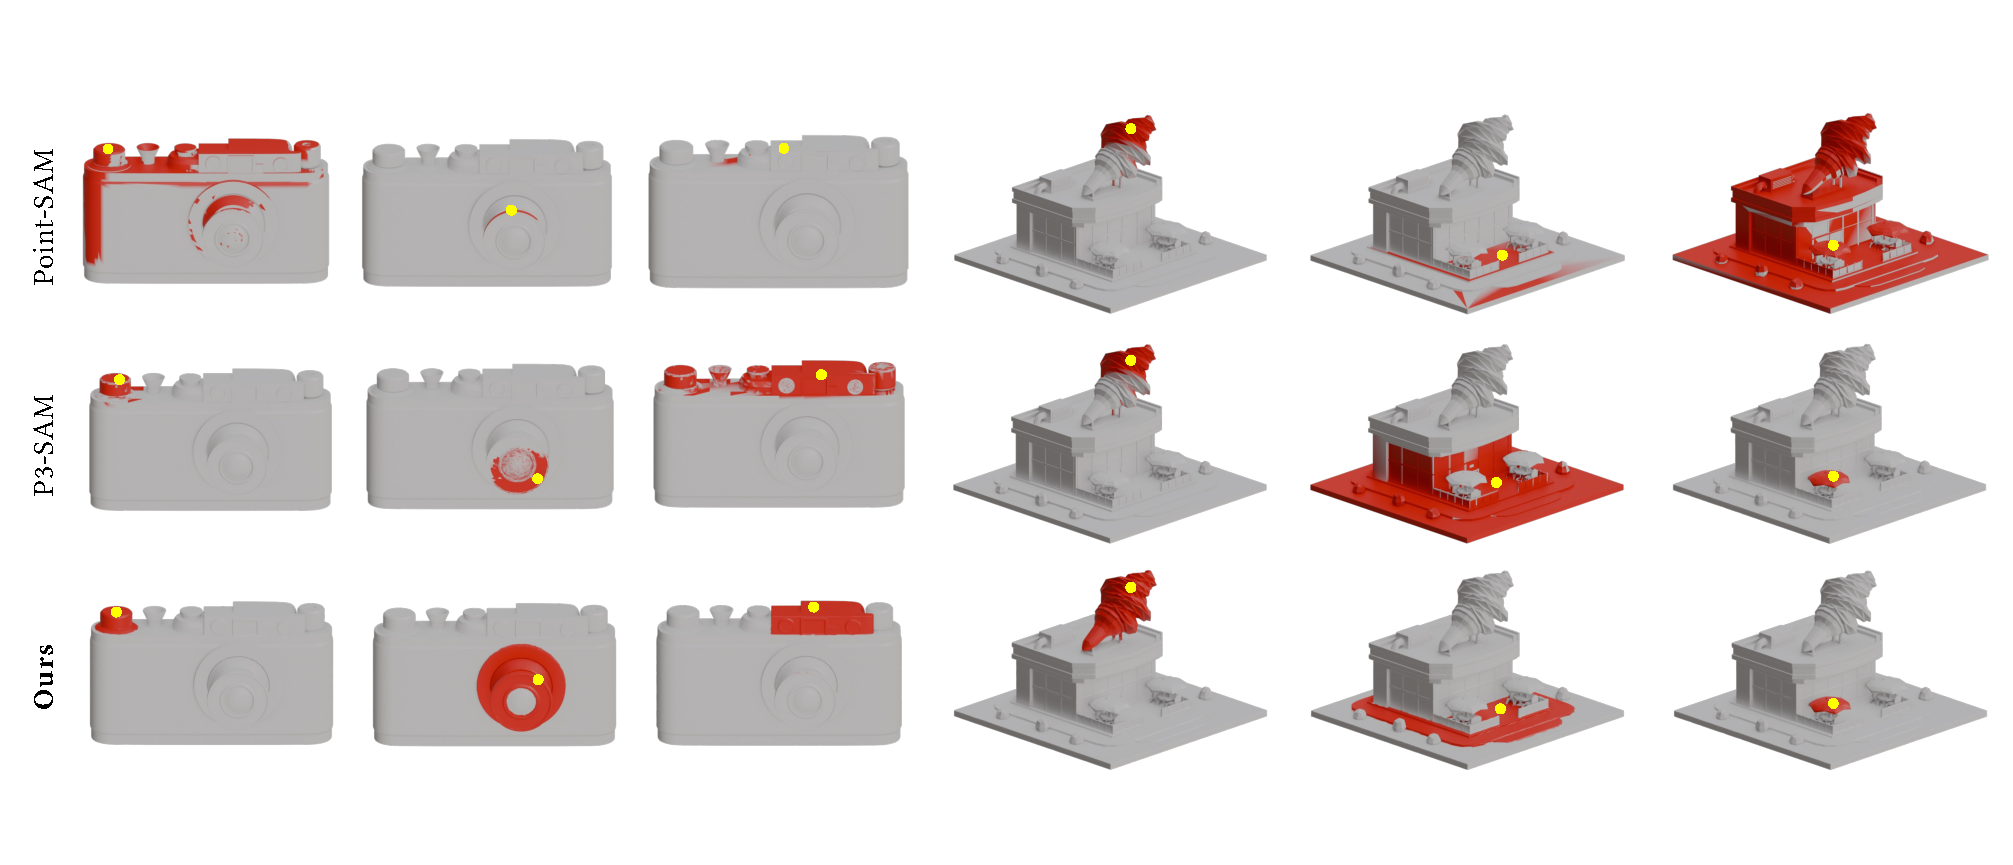
\includegraphics[width=\linewidth]{img/comparison_point.pdf}
  \caption{
  Interactive part-segmentation results. 
  %
  We compare \textit{SegviGen} with existing representative baselines, including Point-SAM~\cite{pointsam} and P3-SAM~\cite{p3sam}. 
  %
  In the figure, yellow points denote user clicks, while the predicted target part is highlighted in red.
  %
  Leveraging priors from pretrained 3D generative models, \textit{SegviGen} achieves more accurate results with sharper boundaries than prior methods, while requiring substantially less training data.
  }
  \label{fig:comparison_point}
\end{figure*}


\paragraph{Condition Injection.}
We adopt task-specific conditioning designs while maintaining a unified interface across settings.
%
For interactive segmentation, user clicks in the UI provide an efficient and intuitive form of guidance.
%
In our framework, each click is encoded as a sparse point token comprising its 3D coordinates and an associated feature vector.
%
Since the 3D coordinates are already effectively encoded by RoPE within the attention layers, 
%
we omit the additional learnable input-level positional embedding used in prior designs~\cite{p3sam}.
%
Instead, all points share the same learnable feature vector $Q$ , which serves as the point token during both training and inference.
%
Given point coordinates $\mathbf{u}=\{u_i\}_{i=1}^{m}$ with $u_i\in\mathbb{R}^3$, we form point-condition tokens
\begin{equation}
Q \;=\; \big[\; \mathbf{q}(u_1),\ldots,\mathbf{q}(u_m) \;\big], 
\quad
\mathbf{q}(u_i) \;=\; \big[\, u_i \,;\, \mathbf{e}_p \,\big],
\end{equation}
where $\mathbf{e}_p$ is a shared learnable feature appended to every point token.
%
Conditioned on $Q$, the denoising model is instantiated as
\begin{equation}
\hat{v}_{\theta} \;=\; f_{\theta}\!\left(y_t,\, z,\, Q,\, e_{\tau},\, t\right).
\end{equation}
%
When the number of points is fewer than $10$, we pad the point tokens to a length of $10$
using zero coordinates and zero features.
%
To preserve a single unified model, we keep this interface for full segmentation and 2D-guided full segmentation by providing $10$ padded tokens with all-zero coordinates and features.


For full segmentation with 2D guidance, we additionally provide a user-specified 2D segmentation colorization as guidance, allowing direct control over the desired part granularity and label palette.
%
The guidance image is encoded into a sequence of conditioning tokens injected via cross-attention:
\begin{equation}
p \;=\; g_{\phi}(I_{\text{guide}}),
\end{equation}
where $g_{\phi}(\cdot)$ denotes an image encoder.
%
In this setting, denoising is conditioned on both the padded point-token interface $Q_{0}$ and the image guidance tokens $p$:
\begin{equation}
\hat{v}_{\theta} \;=\; f_{\theta}\!\left(y_t,\, z,\, (Q_{0},\, p),\, e_{\tau},\, t\right).
\end{equation}

\paragraph{Task Embedding.}
To improve multi-task generalization within a single model, task identity is encoded as a continuous embedding and injected alongside the timestep signal.
%
Let $\tau\in\{1,\dots,T\}$ denote the task index.
%
A sinusoidal encoding is first computed from $\tau$,
\begin{equation}
s_{\tau} \;=\; \mathrm{PE}(\tau)\in\mathbb{R}^{d_f},
\end{equation}
where $\mathrm{PE}(\cdot)$ follows the standard sinusoidal scheme.
%
A lightweight MLP then maps $s_{\tau}$ to the task embedding
\begin{equation}
e_{\tau} \;=\; \mathrm{MLP}_{\psi}(s_{\tau}) \in \mathbb{R}^{d}.
\end{equation}
In parallel, the timestep $t$ is embedded as $e_t\in\mathbb{R}^{d}$.
The final modulation vector used by DiT backbone is obtained by additive fusion,
\begin{equation}
m \;=\; e_t \;+\; e_{\tau},
\qquad
\hat{v}_{\theta} \;=\; f_{\theta}\!\left(y_t,\, z,\, C,\, m\right),
\end{equation}
where $m$ conditions the adaptive layers to jointly encode diffusion progress and task semantics.
%
During training, samples from different tasks are interleaved and supervised with their corresponding $\tau$, 
encouraging the shared backbone to learn task-discriminative behaviors while preserving a unified parameterization.










